\begingroup
\emergencystretch=1em
\section{Bounded evaluation: draft pending independent review}
\label{sec:bounded-evaluation}
\textbf{Full manuscript gate: BLOCKED.} These tables describe separate,
independently admitted evidence slices, not a completed nine-graph comparison.
Their assembly and presentation in this draft still require independent review.
Source admission does not establish novelty. No broad superiority, speedup,
noise resilience, or device compatibility follows. Evidence identifiers E1--E6
refer to the dated claim ledger and its SHA256 source index.

\subsection{Matched components and the comparison denominator (E1)}
The saved continuation covers myciel5 and 2-Insertions\_3, R1--R3, iteration
$j=1$, seed 7, and the recorded method/profile contexts. Only the exact
preparation/diffusion intersection supports unrestricted component reuse within
the reviewed construction. Neither a finite witness test nor an accounting
recount proves the larger compiled predicates on all inputs.
\begin{table}[t]
\caption{Logical comparison admission. Rows, matched metric details, and
summaries have different denominators. Shared components show no advantage.}
\label{tab:bounded-comparison}
\centering\small
\begin{tabular}{lr}\toprule
Admitted preparation/diffusion rows & 230\\
Matched metric details: wins / ties / losses & 0 / 492 / 0\\
Summary groups over those details & 378\\
All-input oracle/search comparison rows admitted & 0\\\bottomrule
\end{tabular}
\end{table}
The wider descriptive arithmetic has 84 wins, 492 ties, and 408 losses in
984 metric details. Its wins and losses are sample-qualified oracle/search
diagnostics, excluded from unrestricted comparative conclusions. Raw primitive
costs, missing compilation identities, mixed representations, and other targets
cannot extend Table~\ref{tab:bounded-comparison}. No geometric mean over these
incompatible slices is reported.

\subsection{Ideal C5 iteration sweep and overshoot (E2)}
For the unprecolored five-cycle with three colors, direct enumeration gives
$M=30$ proper colorings. R1 prepares all $N=1024$ binary words; R2 prepares
$N=243$ valid-code words. Both retain the complete predicate and use the actual
emitted preparation inverse in the matching reflection. The saved best-fit
phase oracle allocates 11 wires, including ten data wires, and contains
84,441 logical U/CX instructions. This width is not a gate-cost advantage.
\begin{table}[t]
\caption{Saved ideal C5/k3 observations, not shots. All ten agree with
analytical amplitude amplification within $10^{-10}$.
R2 has fewer iterations but a lower discrete first peak.}
\label{tab:bounded-c5}
\centering\small
\begin{tabular}{crrr}\toprule
Regime & $j$ & Proper success & Unused-code probability\\\midrule
\csname @@input\endcsname bounded-evaluation-20261113/c5-rows.tex
\bottomrule\end{tabular}
\end{table}
R1 peaks at $j=4$ with success 0.999484622397, then falls to
0.900260183699. R2 peaks at $j=2$ with 0.950509084831, then falls to
0.345567160993. R1 intentionally starts with unused codes; at its peak their
probability is 0.000404939543798. R2's observed unused-code probability remains
below $1.98\times10^{-27}$. These deterministic complex128 observations have
no binomial confidence interval; residuals are numerical checks, not rigorous
error bounds. Transpiler seed 7 is fixed; no scientific sampling reran here.
\begin{figure*}[t]
\centering
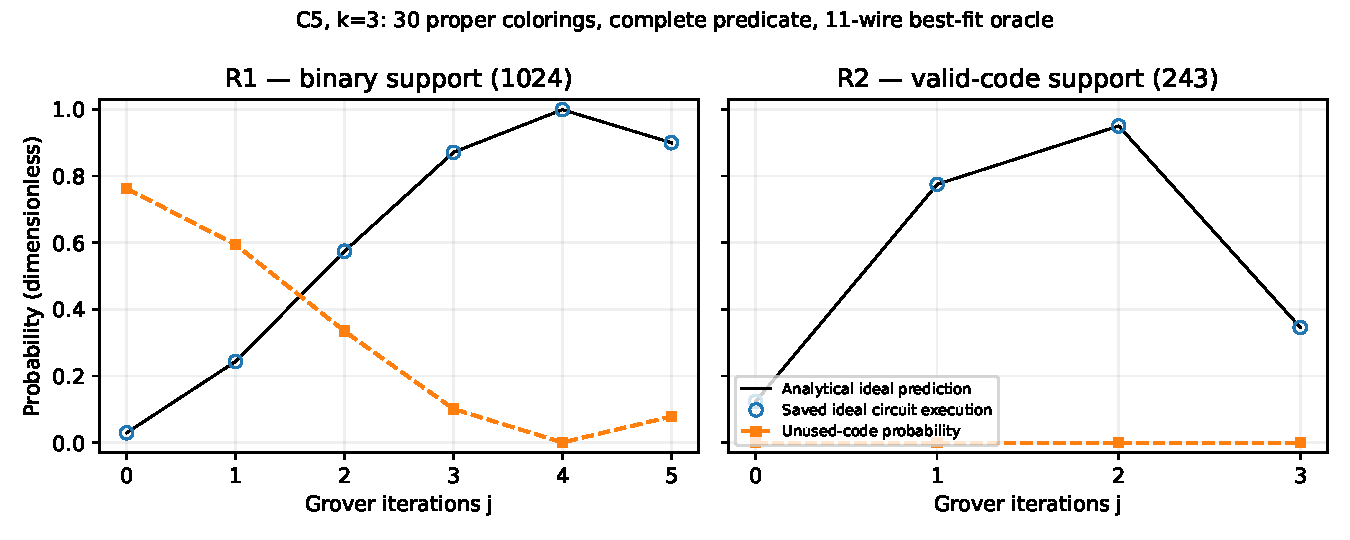
\includegraphics[width=.95\textwidth]{bounded-evaluation-20261113/assets/c5-admitted-iterations.pdf}
\caption{C5/k3, complete predicate, saved 11-wire best-fit oracle. Open circles
are ten previously executed ideal-state observations; black segments connect
analytical predictions at integer iterations, not continuous-time trajectories.
Orange squares show unused-code probability. The two panels have different
iteration ranges and a common probability scale. First-peak overshoot decreases
success in both regimes; R2's first peak is lower. The 84,441 U/CX instructions
are logical oracle instructions, not T gates or routed two-qubit gates.
No noise, FT, baseline advantage, or 22-wire structure-pilot admission is implied.
Source CSV, original plotting script, hashes, and exact result/QPY identities
accompany this draft. Presentation admission remains pending.}
\label{fig:bounded-c5}
\end{figure*}
The distinct original 22-wire structure pilot supplies only saved $j=0,1$
observations. Its exact 977-instruction lowered oracle remains pending an
independent clean-data absolute-phase/restoration proof under the assigned
handoff. It is excluded from this figure and no wider numerical replay occurs.

\subsection{Whole-circuit MCX coverage (E3)}
The admitted selected study has 1,608 completed cost rows (189 isolated and
1,419 whole cases), with 42 exclusions. Exactly 1,335 whole cases have bounded
coherent checks; the other 84 whole cost rows lack full statevector validation.
Nine Gray-code exclusions cover 12--20 controls and 33 exclusions concern the
known sb\_original triangle failure. Gray 11 was executed. Dutta trade-offs
remain analytical rather than executed circuits. Peak held scratch is counted
once and cleanup uses the actual expanded inverse; restoring policies replace
unmirrored throwaway marking/reflection. The 5,160 matched-clean-tree metric
diagnostics include 1,411 wins, 2,555 ties, and 1,194 losses. They are not
independent trials or a universal policy ranking. Residual rotations remain
unpriced, so total FT T-count/T-depth/precision are unavailable.

\subsection{Static full-search T costs on one edge (E4)}
The graph has vertices 7 and 11, edge $(7,11)$, three colors, LSB-first inputs,
xag\_bennett, no preprocessing, restoring Gray-code MCX and clean workspace.
R1/R2 use the complete predicate; R3 removes domain checks and retains its
own numeric target. Costs use actual emitted Clifford+$T$ circuits and a
whole-search primary budget $10^{-3}$, with actual emitted $A^\dagger$ reuse.
\begin{table}[t]
\caption{One-edge static FT observations at matched $j=1$, primary precision.
T-depth follows shared-wire dependencies, not an additive component formula.}
\label{tab:bounded-ft}\centering\small
\begin{tabular}{crrr}\toprule
Regime & Wires & Full T-count & Dependency T-depth\\\midrule
R1 & 13 & 271982 & 194958\\
R2 & 13 & 353792 & 222800\\
R3 & 7 & 353624 & 222764\\\bottomrule
\end{tabular}
\end{table}
At this matched schedule, valid preparation loses 81,810 T (R2) or 81,642 T
(R3) relative to R1. The accounting is
$T_A+j(2T_A+T_O+T_{S_0})$: R1 uses $0+182+271800$;
R2 uses $3(27270)+182+271800$; R3 substitutes $14$ for $182$.
There are 12 completed study rows plus one identical-circuit final-source smoke.
Three $j=1$, $10^{-4}$ sensitivity attempts failed the fixed bounded rotation
synthesis and retain null search costs. They are not analytical replacements.
First-peak schedules differ: valid preparation peaks at $j=0$, while R1 peaks
at $j=1$. The $j=0$ primary valid preparation costs 5,810 T but invokes no
oracle. H preparation at $j=0$ already gives $3/8$ proper success at zero T.
Verification, Clifford and runtime costs are unpriced; achieved preparation
break-even remains null. These are numerical clean-subspace observations,
not a general approximation or dirty-workspace theorem.

\subsection{Separate finite-cap dynamic RUS evidence (E5)}
For one uncontrolled two-bit vertex register, with ideal fresh-zero retry
ancilla and noiseless classical control, cap four gives completion
$q=1-4^{-4}=255/256$. Expected reached attempts are
$a=1+1/4+1/16+1/64=1.328125$. Unconditional stop costs, including aborts,
are $2a+2q=4.6484375$ T forward and $2a+2=4.65625$ T inverse.
The inverse prefix occurs once even at cap zero. These expectations agree with
the separately admitted 20 finite-cap cases/220 terminal branches; they are
not static circuit T-counts. Non-T operations are unpriced. No graph search,
quantum control, or substitution for static $A/A^\dagger$ is admitted by this
slice. A naive controlled construction yields purity 0.8125 after records are
discarded, which is an explicit obstruction to that substitution. The analytical
unlimited $14/3$ limit is not unlimited execution evidence.

\subsection{Conditional noisy observations and unfavorable counts (E6)}
The original admitted pilot comprises 28 fixed 64-shot records, totaling
1,792 shots: 15 path3/k2 R1 and 13 K3/k3 R2 records. Each uses the saved
FakeTorino gate/readout/per-gate thermal model and routing seeds
11/23/37/41/53; idle relaxation, drift, and crosstalk are excluded.
At K3 R2 $j=1$, proper counts are respectively 3,10,10,3,7 out of 64;
unused-code counts are 37,28,24,34,33. These unfavorable conditional observations
do not support noise resilience. At $j=2$, seed23 is 21-wire excluded and
seed37 has no admitted counts in this pilot. Saved pointwise Wilson 95\%
intervals apply per fixed circuit, with no simultaneous or seed-pooled coverage.
Native two-qubit gates/proper output and classical draws plus predicate
evaluation/proper output have unlike units; they establish no speedup.

The later 9 November family admission is a distinct source generation:
376 additional conditional histograms/24,064 shots, retaining the original
28/1,792. Thus 404 request records/25,856 shots are admitted across generations,
and $805-404=401$ frozen keys lack admitted family observations at that admission.
This is an inventory total, not pooled replications. K3 R1 $j=2$, seed11 returned
4/64 proper outputs (pointwise Wilson 95\%: 2.46--15.00\%) versus saved ideal
99.9779\%, with 37/64 unused codes. A histogram missing its terminal receipt
stays withheld. These admissions license neither C5 noise nor complete families.

\subsection{Excluded and unrun scope}
The full matched nine-graph R1--R3 study, strongest-baseline rankings, common
lowering, five-seed routing, full precision/MCX/profile ablations, larger CEC,
selected/full-DIMACS five-repeat scaling, complete noisy first-lobe sweeps,
graph-level coherent RUS and achieved success-cost break-even are not supplied
by these tables. They remain separately gated; no missing row is imputed.
The structure22 lowering proof remains pending under the assigned handoff.
Hardware, physical QEC, precolored instances and conditional-workspace synthesis
remain excluded. These bounded checks can support a future comparative study;
they cannot yet choose its final title, abstract, contributions or conclusions.
\endgroup
